\documentclass[12pt,a4paper]{article}
\usepackage[utf8]{inputenc}
\usepackage[russian]{babel}
\usepackage[OT1]{fontenc}
\usepackage{graphicx}
\usepackage[left=1cm,right=1cm,top=1cm,bottom=1cm]{geometry}
\author{Владимир Журавлев}
\usepackage{pgfplots}
\usepackage{graphicx}
\usepackage{amsmath}
\pgfplotsset{compat=1.9}
\pagestyle{plain}
\usepackage{pgfplotstable,filecontents}

\begin{document}
\begin{flushright}

\textbf{Журавлев Владимир, 621 гр.\\}


\end{flushright}
\begin{center}
\begin{LARGE}

\vspace{\baselineskip}
Лабораторная работа №4.5.2\\
\textbf{
ИНТЕРФЕРЕНЦИЯ
ЛАЗЕРНОГО ИЗЛУЧЕНИЯ}\\
\vspace{\baselineskip}

\end{LARGE}
\end{center}
\section{Немного теории}
Лазер работает на волнах 
\[\lambda_0 = 632.8 nm \]
Доплеровский эффект вызывает уширение спектральной линии, в приближении небольших скоростей и разложении по линейным членам $\frac{v}{c}$ релятивистких эффектов позволяет нам говорить о максвелловском виде спектра. Характерной особенностью является очень узкая величина уширения и соответственно небольшое количество возбужденных побочных мод в лазерном резонаторе. 

\[\Delta f = f_0 \sqrt{\frac{2kT}{mc^2}} \]


\section{Измерение коэффициента видности}

Коэффициент видности зависит от нескольких величин, примем без доказательства, что суммарный коэффициент можно представить в виде:
\[\gamma = \gamma_1 \gamma_2 \gamma_3 \]
\subsection{Разные амплитуды монохроматических волн }

Видность (1) обусловлена видностью одной моды излучения частоты $f_m$ для волн разных амплитуд, сходящихся под маленьким углом  с разностью хода $l$:
\[ \Delta = k_m l  = \frac{2 \pi}{\lambda} l\]
\[ I = A_m^2 + B_m^2 + 2A_m B_m \cos (\Delta) \]

В минимуме и максимуме можно выразить видность через безразмерный параметр $\delta \equiv\delta_m = A^2_m / B^2_m$ 

\[ \gamma_1 = \frac{2\sqrt{\delta}}{1+\delta} \]

Т.е. видность (1) определяется только амплитудами интерферирующих волн.\\
\subsection{Рассмотрение влияния нескольких мод колебаний}
Пренебрегая межмодовыми биениями, можно рассмотреть интенсивность суммарной волны как сумму интенсивностей интерферирующих мод:
\[I = \sum \limits_{m} A^2_m(1+\delta + 2\sqrt{\delta} \cos ( \frac{2 \pi}{\lambda_m} l)) \]

Функция представляет собою часть тригонометрического ряда, максимум суммы которого достигается при условии:
\[ \Delta_m  =  pi \frac{l}{L} = 2 \pi n_m \]
Откуда получаем, что максимум будет при $l = \pm (2k) L$\\

Определяя форму $\gamma_2$ можно найти связь полуширины $\gamma_2$ c $\Delta F$:
\[ l_{1/2} = \frac{c}{\pi \Delta F} \sqrt{\ln 2} \approx \frac{0.26 c}{\Delta F} \]

\subsection{Поляризация}

В интерференции принимают участие волны с одинаковой поляризацией. Вклад различной поляризации линейных волн:
\[\gamma_3 = | \cos \alpha| \]

\section{Ход работы}
Измерения производятся с помощью осциллографа, по сигналу которого мы сразу можем измерить видность картины. Сначала исследуем зависимость $\gamma_3 (\alpha)$. Чтобы легче пронаблюдать ожидаемую зависимость лучше строить график $\gamma_3 \cos (\alpha)$, предполагая зависимость вида $\gamma_3 = |t|$\\

\begin{center}
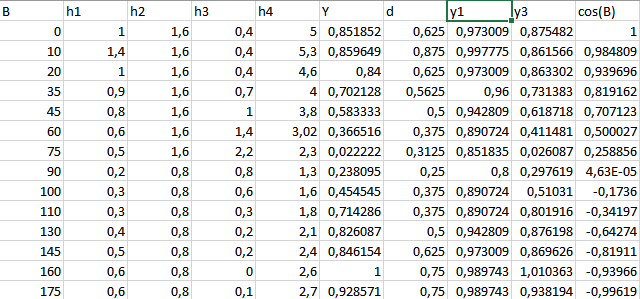
\includegraphics[scale=1]{452_tables.png}
\end{center}
\begin{center}
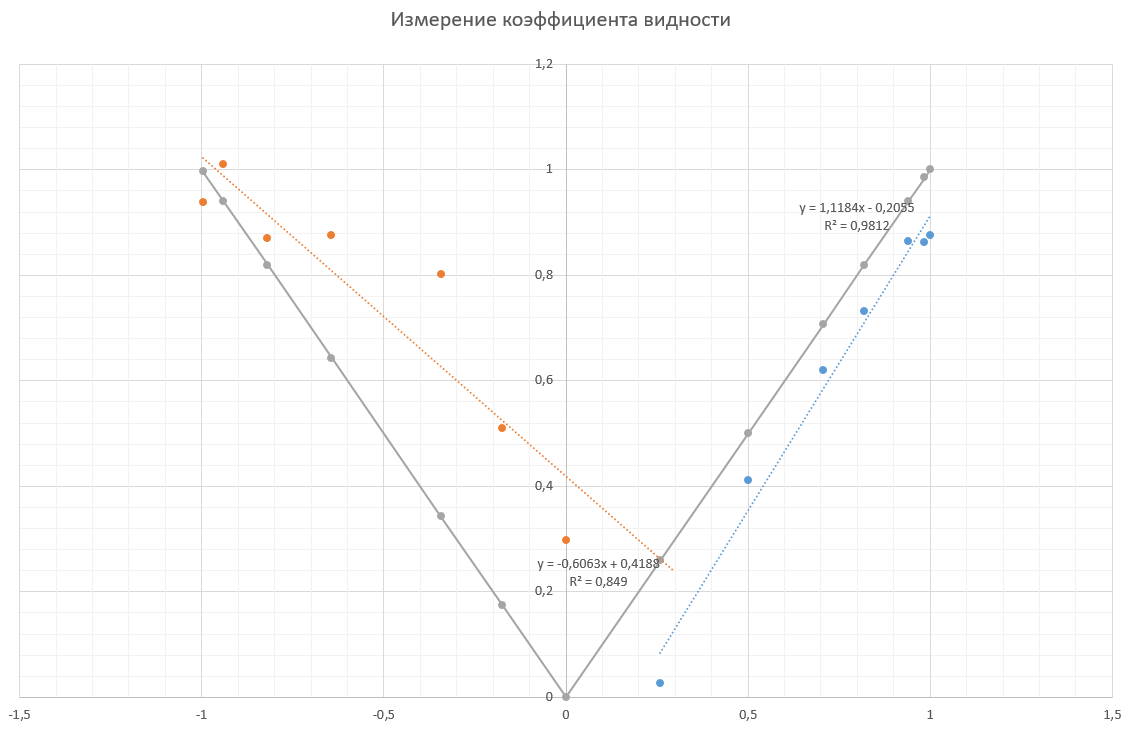
\includegraphics[scale=0.6]{452_graph1.png}
\end{center}


Теперь установим зависимость $\gamma_2$
Будем двигать штангу вдоль оси и честно снимать точки
\begin{center}
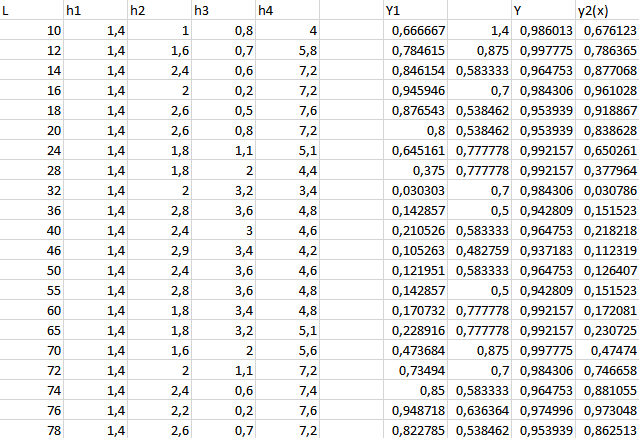
\includegraphics[scale=1]{452_tables2.png}
\end{center}

\begin{center}
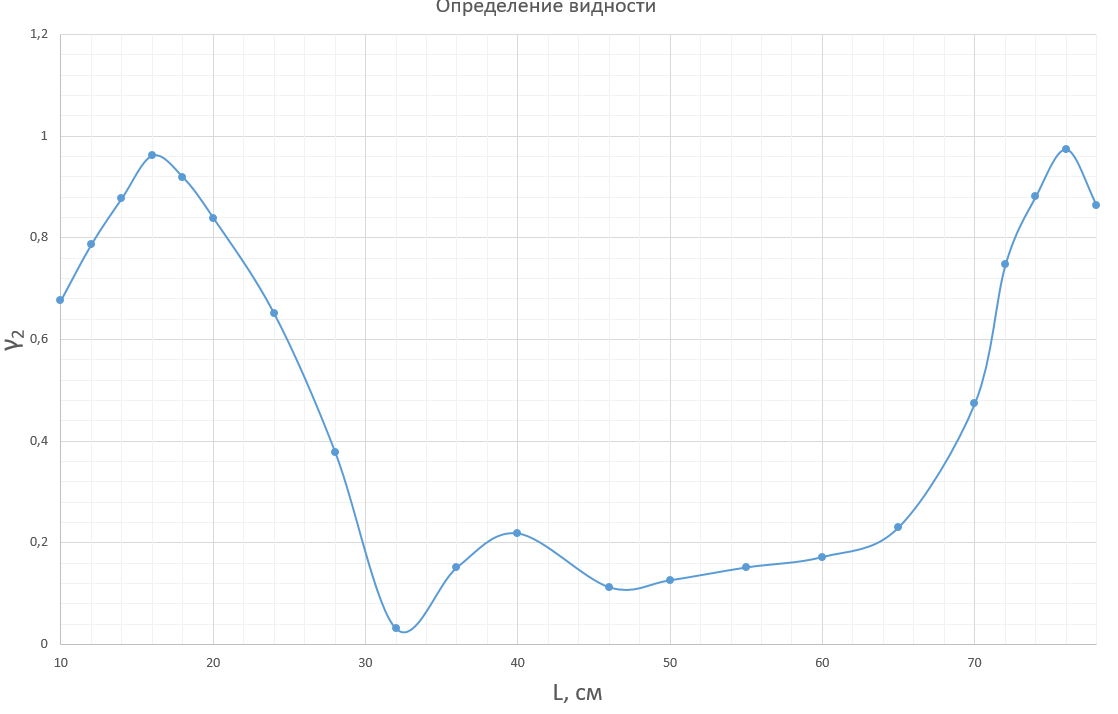
\includegraphics[scale=0.6]{452_graph2.png}
\end{center}
 
Отсюда по расстоянию между максимумами можно найти длину лазера:
\[L = 30 \pm 2 \; cm.\]
И оценить ширину спектра:
\[\Delta F = \frac{0.26 c}{[l_{1/2} = 11cm]} \approx (7,1 \pm 0,7) \cdot 10^8  \; hz\]
Число мод:
\[N = 1 + 2 \frac{\Delta F}{\Delta \nu} = 1 + 2 \frac{7}{5} \approx 3 \pm 1 \]



\end{document}